\documentclass{article}
  
%package list
\usepackage[top=3cm, bottom=3cm, outer=3cm, inner=3cm]{geometry}
\usepackage{multicol}
\usepackage{graphicx}
\usepackage{url}
%\usepackage{cite}
\usepackage{hyperref}
\usepackage{array}
%\usepackage{multicol}
\usepackage{natbib}
\usepackage{pdfpages}
\usepackage{multirow}
\usepackage[normalem]{ulem}
\useunder{\uline}{\ul}{}
\usepackage{svg}
\usepackage{xcolor}
\usepackage{listings}
\usepackage{csquotes}
%\usepackage{booktabs}
\usepackage{caption}
\usepackage{subcaption}
\usepackage{float}
\usepackage{array}
\usepackage{comment} 				% Para comentar
\usepackage[english,spanish]{babel}
\usepackage[utf8]{inputenc}


\newcolumntype{x}[1]{>{\centering\arraybackslash\hspace{0pt}}p{#1}}
\newcolumntype{M}[1]{>{\centering\arraybackslash}m{#1}}
\newcolumntype{N}{@{}m{0pt}@{}}

  
% Items de comand
%%%%%%%%%%%%%%%%%%%%%%%%%%%%%%%%%%%%%%%%%%%%%%%%%%%%%%%%%%%%%%%%%%%%%%%%%%%%
%%%%%%%%%%%%%%%%%%%%%%%%%%%%%%%%%%%%%%%%%%%%%%%%%%%%%%%%%%%%%%%%%%%%%%%%%%%%
\newcommand{\itemEmail}{}
\newcommand{\itemStudent}{
Jhonatan Benjamin Mamani Céspedes
y Álvaro Raúl Quispe Condori}
\newcommand{\itemCourse}{Práctica}
\newcommand{\itemCourseCode}{20230467}
\newcommand{\itemSemester}{II}
\newcommand{\itemUniversity}{Universidad Nacional de San Agustín de Arequipa}
\newcommand{\itemFaculty}{Facultad de Ingeniería de Producción y Servicios}
\newcommand{\itemDepartment}{Departamento Académico de Ingeniería de Sistemas e Informática}
\newcommand{\itemSchool}{Escuela Profesional de Ingeniería de Sistemas}
\newcommand{\itemAcademic}{2023 - B}
\newcommand{\itemInput}{14 de enero}
\newcommand{\itemOutput}{16 de enero}
\newcommand{\itemPracticeNumber}{02}
\newcommand{\itemTheme}{Bases de Datos}

\AtBeginDocument{\selectlanguage{spanish}}
\renewcommand{\figurename}{Figura}
\renewcommand{\refname}{Referencias}
\renewcommand{\tablename}{Tabla} %esto no funciona cuando se usa babel
\AtBeginDocument{%
	\renewcommand\tablename{Tabla}
}

  
% Set

\lstdefinestyle{ascii-tree}{
    literate={├}{|}1 {─}{--}1 {└}{+}1 
  }
\lstset{basicstyle=\ttfamily,
  showstringspaces=false,
  commentstyle=\color{red},
  keywordstyle=\color{blue}
}
\lstset{										%Para código
  literate=
  {á}{{\'a}}1 {é}{{\'e}}1 {í}{{\'i}}1 {ó}{{\'o}}1 {ú}{{\'u}}1
  {Á}{{\'A}}1 {É}{{\'E}}1 {Í}{{\'I}}1 {Ó}{{\'O}}1 {Ú}{{\'U}}1
  {ã}{{\~a}}1 {ẽ}{{\~e}}1 {ĩ}{{\~i}}1 {õ}{{\~o}}1 {ũ}{{\~u}}1
  {Ã}{{\~A}}1 {Ẽ}{{\~E}}1 {Ĩ}{{\~I}}1 {Õ}{{\~O}}1 {Ũ}{{\~U}}1
	{ñ}{{\~n}}1 {Ñ}{{\~N}}1 
}
\lstset{frame=tb,
	language=bash,
	aboveskip=3mm,
	belowskip=3mm,
	showstringspaces=false,
	columns=flexible,
	basicstyle={\small\ttfamily},
	numbers=none,
	numberstyle=\tiny\color{gray},
	keywordstyle=\color{blue},
	commentstyle=\color{dkgreen},
	stringstyle=\color{mauve},
	breaklines=true,
	breakatwhitespace=true,
	tabsize=3,
	backgroundcolor= \color{codebackground},
}
% para el codigo fuente
\usepackage{listings}
\usepackage{color, colortbl}
\definecolor{dkgreen}{rgb}{0,0.6,0}
\definecolor{gray}{rgb}{0.5,0.5,0.5}
\definecolor{mauve}{rgb}{0.58,0,0.82}
\definecolor{codebackground}{rgb}{0.95, 0.95, 0.92}
\definecolor{tablebackground}{rgb}{0.8, 0, 0}

  
%Al parecer encabezado
\usepackage{fancyhdr}
\pagestyle{fancy}
\fancyhf{}
\setlength{\headheight}{42pt}
\renewcommand{\headrulewidth}{1pt}
\renewcommand{\footrulewidth}{1pt}
\fancyhead[L]{\raisebox{-0.2\height}{
\includegraphics[width=3cm]{img/logo_episunsa.png}}}
\fancyhead[C]{\fontsize{7}{7}\selectfont	\itemUniversity \\ \itemFaculty \\ \itemDepartment \\ \itemSchool \\ \textbf{\itemCourse}}
\fancyhead[R]{\raisebox{-0.2\height}{
\includegraphics[width=1.2cm]{img/logo_abet}}}
\fancyfoot[L]{}
\fancyfoot[C]{\itemCourse}
\fancyfoot[R]{Página \thepage}


\begin{document}

  
	\vspace*{10px}
% Desde aquí empieza el título
	\begin{center}	
	\fontsize{17}{17} \textbf{ Informe: práctica \itemPracticeNumber}
	\end{center}
	\centerline{\textbf{\Large Tema: \itemTheme}}
	%\vspace*{0.5cm}	

	\begin{flushright}
		\begin{tabular}{|M{2.5cm}|N|}
			\hline 
			\rowcolor{tablebackground}
			\color{white} \textbf{Nota}  \\
			\hline 
			     \\[30pt]
			\hline 			
		\end{tabular}
	\end{flushright}	

	\begin{table}[H]
		\begin{tabular}{|x{4.7cm}|x{4.8cm}|x{4.8cm}|}
			\hline 
			\rowcolor{tablebackground}
			\color{white} \textbf{Estudiantes} & \color{white}\textbf{Escuela}  & \color{white}\textbf{Asignatura}   \\
			\hline 
			{\itemStudent \par \itemEmail} & \itemSchool & {\itemCourse \par Semestre: \itemSemester \par Código: \itemCourseCode}     \\
			\hline 			
		\end{tabular}
	\end{table}		
	
	\begin{table}[H]
		\begin{tabular}{|x{4.7cm}|x{4.8cm}|x{4.8cm}|}
			\hline 
			\rowcolor{tablebackground}
			\color{white}\textbf{Práctica} & \color{white}\textbf{Tema}  & \color{white}\textbf{Duración}   \\
			\hline 
			\itemPracticeNumber & \itemTheme & 04 horas   \\
			\hline 
		\end{tabular}
	\end{table}
	
	\begin{table}[H]
		\begin{tabular}{|x{4.7cm}|x{4.8cm}|x{4.8cm}|}
			\hline 
			\rowcolor{tablebackground}
			\color{white}\textbf{Semestre académico} & \color{white}\textbf{Fecha de inicio}  & \color{white}\textbf{Fecha de entrega}   \\
			\hline 
			\itemAcademic & \itemInput &  \itemOutput  \\
			\hline 
		\end{tabular}
	\end{table}


%%%%%%%%%%%%%%%%%%%%%%%%%%%%%%%%%%%%%%%%%%%%%%%%%
%%%%%%%%%%%%%%%%%%%%%%%%%%%%%%%%%%%%%%%%%%%%%%%%%
% Actividades------------------------------------
	\section{Actividades}
	\begin{itemize}		
    \item Crear una base de datos con MARIADB.
		\item Conectarse a una base de datos con java.
    \item Usar Singleton para conectarse con un único objeto.
  \end{itemize}
%%%%%%%%%%%%%%%%%%%%%%%%%%%%%%%%%%%%%%%%%%%%%%%%%
%%%%%%%%%%%%%%%%%%%%%%%%%%%%%%%%%%%%%%%%%%%%%%%%%
% Equipo-----------------------------------------

	\section{Equipos, materiales y temas empleados}
	\begin{itemize}
		\item Sistema Operativo POP os, 22.04 LTS.
		\item NVIM 0.6.1.
		\item OpenJDK 64-Bits 17.0.7.
		\item Git 2.39.2.
		\item Cuenta en GitHub con el correo institucional.
		\item Programación Orientada a Objetos.
	\end{itemize}

%%%%%%%%%%%%%%%%%%%%%%%%%%%%%%%%%%%%%%%%%%%%%%%%%
%%%%%%%%%%%%%%%%%%%%%%%%%%%%%%%%%%%%%%%%%%%%%%%%%
% Repositorio------------------------------------
	\section{URL de Repositorio Github y video-grabación}
	\begin{itemize}
		\item URL del Repositorio GitHub para clonar o recuperar.
		\item \url{https://github.com/ALVARO-QUISPE-UNSA/fp2-23b}
		\item URL para la práctica 02 en el Repositorio GitHub.
		\item \url{https://github.com/ALVARO-QUISPE-UNSA/fp2-23b/tree/main/fase03/prac02}
		\item URL para la grabación de la compilación
		\item \url{https://drive.google.com/file/d/1CE_5pEXvPoFedSczyST0HGrHY-bEKgYR/view?usp=sharing}
	\end{itemize}
%%%%%%%%%%%%%%%%%%%%%%%%%%%%%%%%%%%%%%%%%%%%%%%%%
%%%%%%%%%%%%%%%%%%%%%%%%%%%%%%%%%%%%%%%%%%%%%%%%%
% Desarrollo de actividad------------------------

  \section{Desarrollo de la actividad}


% ----------------------Subseccón----------------
  \subsection{Conexión a la base de datos}
  \begin{itemize}
    \item Se ha escrito un programa en Java que utiliza el controlador JDBC de MySQL para establecer una conexión con una base de datos MariaDB local.
    \item La clase \texttt{Class.forName("com.mysql.cj.jdbc.Driver")} se ha empleado para cargar el controlador JDBC necesario para la conexión.
    \item La URL de conexión se ha definido como jdbc : mysql://localhost:3306/fp2-23b, especificando la dirección del servidor, el puerto y el nombre de la base de datos.
    \item Se han proporcionado las credenciales de usuario (\texttt{user}) y contraseña (\texttt{password}) para autenticarse en la base de datos.
    \item Se ha utilizado la clase \texttt{SingleDriver} para obtener la conexión mediante el método \texttt{getDriver}, aunque la implementación exacta de esta clase no se presenta en el código proporcionado.
  \end{itemize}


      % Codigo--------------
      \begin{lstlisting}[language=Java, caption={Main.java}, numbers=left, firstnumber=1][H]
import java.sql.*;
public class Main {
  public static void main(String args[]) {
    try {
      // Corrección del nombre del controlador 
      Class.forName("com.mysql.cj.jdbc.Driver");

      // Conexión con la base de datos
      String url = "jdbc:mysql://localhost:3306/fp2_23b";
      String user = "fp2_23b";
      String password = "12345678";
      Connection miConexion = SingleDriver.getDriver(url, user, password);

      if (miConexion != null) {
        // Operaciones con la conexión exitosa

        // Declaración y ejecución de la consulta SQL
        String consultas = "SELECT first_name, last_name FROM owners";
        Statement statement = miConexion.createStatement();
        ResultSet resultados = statement.executeQuery(consultas);
        
        // Procesamiento de los resultados
        while (resultados.next()) {
          String firstName = resultados.getString("first_name");
          String lastName = resultados.getString("last_name");
          System.out.println("First Name: " + firstName + ", Last Name: " + lastName);
        }
      } else {
        // Manejo del caso de conexión fallida
        System.out.println("La conexión no se pudo establecer");
      }

    // Manejo de las excepciones
    } catch (SQLException e) {
      System.err.println("\u001B[31mError: \n\u001B[0m" + e);
    } catch (ClassNotFoundException e) {
      System.err.println("\u001B[31mError: \n\u001B[0m" + e);
    }
  }
}
    	\end{lstlisting}

\subsection{Implementación del Modelo Singleton en la Clase \texttt{SingleDriver}}
\begin{itemize}
  \item La clase \texttt{SingleDriver} ha sido diseñada siguiendo el patrón de diseño Singleton, que garantiza la existencia de una única instancia de la conexión a la base de datos.

  \item La instancia única de la conexión (\texttt{driver}) se declara como un campo privado y estático, asegurando que sea accesible a través de la clase y no a través de instancias de la misma.

  \item El constructor de la clase es privado (\texttt{private SingleDriver() {}}), lo que evita la creación de instancias adicionales desde fuera de la clase.

  \item El método estático \texttt{getDriver} se encarga de proporcionar la conexión a la base de datos. Si la conexión aún no ha sido inicializada, se crea una nueva conexión utilizando \texttt{DriverManager.getConnection(url, user, pass)} y se asigna a la instancia única de la conexión. Si la conexión ya existe, se devuelve la instancia existente.

  \item En caso de que ocurra una excepción \texttt{SQLException} durante la obtención de la conexión, se imprime un mensaje de error en la consola y se devuelve \texttt{null} para indicar que ha ocurrido un error en la obtención de la conexión.

  \item En resumen, la implementación del modelo Singleton en la clase \texttt{SingleDriver} asegura que solo exista una instancia de la conexión a la base de datos, proporcionando un mecanismo eficiente y controlado para acceder y gestionar dicha conexión.
\end{itemize}



      % Codigo--------------
      \begin{lstlisting}[language=Java, caption={SingleDriver.java}, numbers=left, firstnumber=1][H]
import java.sql.*;
public class SingleDriver {
  // Una única instancia de la conexión
  private static Connection driver;

  // Constructor privado para evitar instancias adicionales de la clase
  private SingleDriver() {}

  // Método estático para obtener una conexión a la base de datos
  public static Connection getDriver(String url, String user, String pass) {
    try {
      // Si la conexión no ha sido inicializada, crea una nueva conexión
      if (driver == null)
        driver = DriverManager.getConnection(url, user, pass);
      return driver;
    } catch (SQLException e) {
      // Si ocurre un error al intentar obtener la conexión, maneja la excepción
      System.err.println("\u001B[31mError: \n\u001B[0m" + e);
      // Devuelve null para indicar que ha ocurrido un error en la obtención de la conexión
      return null;
    }
  }
}
    	\end{lstlisting}
      % Compilación---------
   		\begin{lstlisting}[language=bash,caption={Compilación y ejecución}][H]
$ javac Main.java
$ java -cp .:/usr/share/java/mysql-connector-java-8.2.0.jar Main 
First Name: George, Last Name: Franklin
First Name: Betty, Last Name: Davis
First Name: Eduardo, Last Name: Rodriquez
First Name: Harold, Last Name: Davis
First Name: Peter, Last Name: McTavish
First Name: Jean, Last Name: Coleman
First Name: Jeff, Last Name: Black
First Name: Maria, Last Name: Escobito
First Name: David, Last Name: Schroeder
First Name: Carlos, Last Name: Estaban
 
			\end{lstlisting}

\begin{comment}

      \begin{figure}[H]
        \centering
        \includegraphics[width=\textwidth]{src/j1.png} 
      \end{figure}

        %--------Compilación
      \begin{figure}[H]
        \centering
        \includegraphics[width=0.5\textwidth]{src/a1.png} 
        \caption{figura tal}
      \end{figure}
\end{comment}






%%%%%%%%%%%%%%%%%%%%%%%%%%%%%%%%%%%%%%%%%%%%%%%%%
%%%%%%%%%%%%%%%%%%%%%%%%%%%%%%%%%%%%%%%%%%%%%%%%%
% Estructura-------------------------------------
    
\clearpage
	\section{Estructura de práctica 2}

%   	\begin{lstlisting}[language=bash,caption={Compilación y ejecución del código}][H]

	\begin{itemize}	
		\item El contenido que se entrega en esta práctica es el siguiente:
	\end{itemize}
	
\begin{lstlisting}[style=ascii-tree]
.
|-- lib
|   |-- mysql-connector-j-8.3.0.jar
|-- Main.java
|-- SingleDriver.java
\end{lstlisting}    




%%%%%%%%%%%%%%%%%%%%%%%%%%%%%%%%%%%%%%%%%%%%%%%%%
%%%%%%%%%%%%%%%%%%%%%%%%%%%%%%%%%%%%%%%%%%%%%%%%%
\clearpage
% Diagrama UML-----------------------------------
  \section{Diagrama UML del proyecto}
    \begin{itemize}	
      \item La estructura del proyecto se refleja en el siguiente diagrama UML
    \end{itemize}
    \begin{figure}[H]
      \centering
      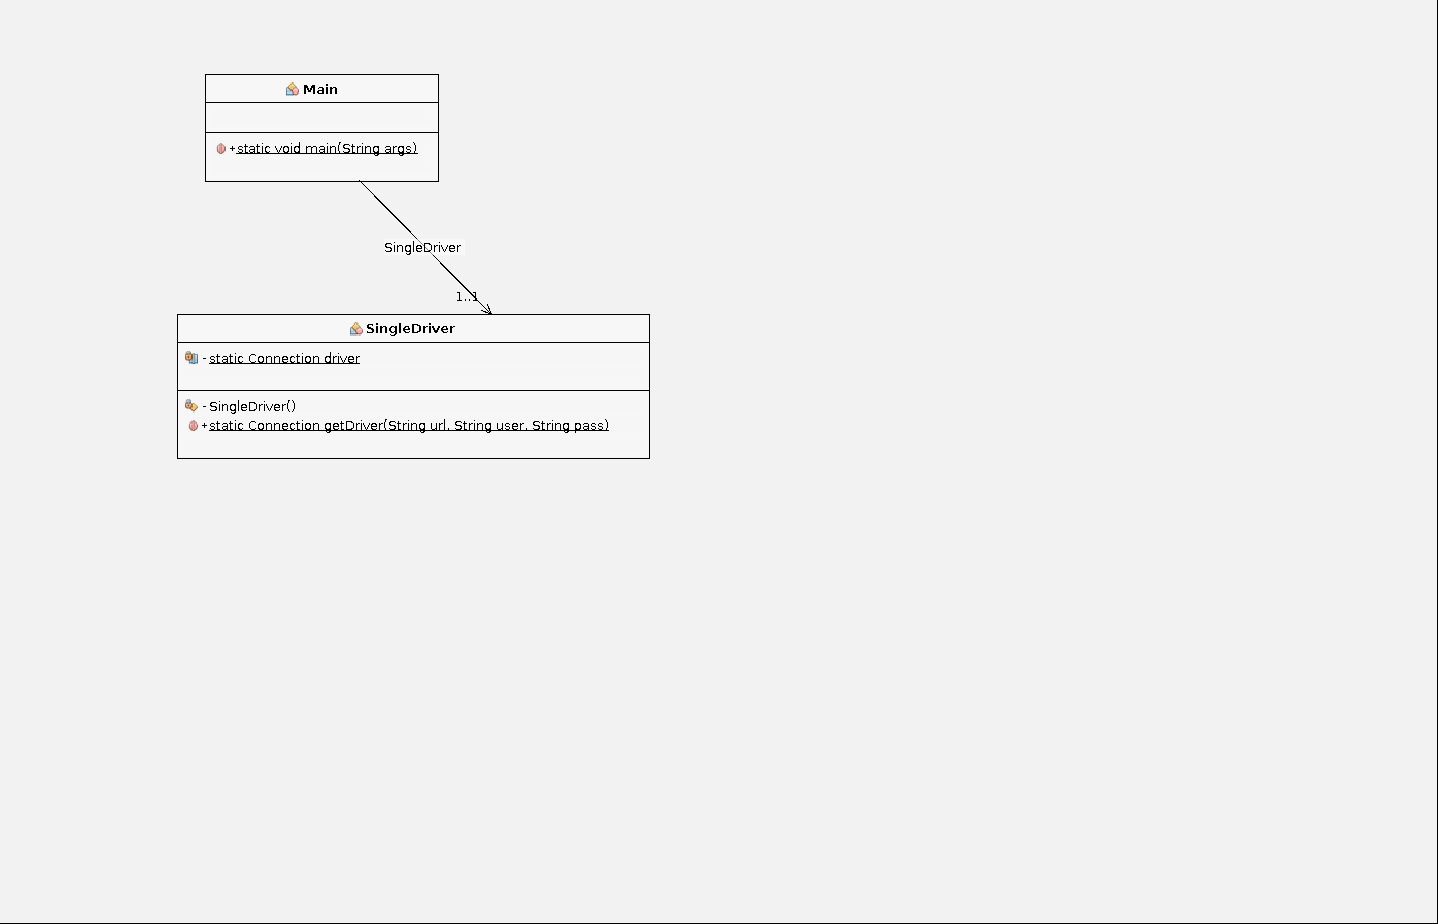
\includegraphics[width=\textwidth]{img/a.png} 
    \end{figure}


%%%%%%%%%%%%%%%%%%%%%%%%%%%%%%%%%%%%%%%%%%%%%%%%%
%%%%%%%%%%%%%%%%%%%%%%%%%%%%%%%%%%%%%%%%%%%%%%%%%
\clearpage
% Referencias------------------------------------
\section{Referencias}
\begin{itemize}			
    \item \url{https://docs.oracle.com/javase/8/docs/api/}
\end{itemize}	
%%%%%%%%%%%%%%%%%%%%%%%%%%%%%%%%%%%%%%%%%%%%%%%%%
%%%%%%%%%%%%%%%%%%%%%%%%%%%%%%%%%%%%%%%%%%%%%%%%%
% Rúbricas---------------------------------------
  
	\section{\textcolor{red}{Rúbricas}}
	
% ----Subseccion------------------------
	\subsection{\textcolor{red}{Entregable Informe}}
	\begin{table}[H]
		\caption{Tipo de Informe}
		\setlength{\tabcolsep}{0.5em} % for the horizontal padding
		{\renewcommand{\arraystretch}{1.5}% for the vertical padding
		\begin{tabular}{|p{3cm}|p{12cm}|}
			\hline
			\multicolumn{2}{|c|}{\textbf{\textcolor{red}{Informe}}}  \\
			\hline 
			\textbf{\textcolor{red}{Latex}} & \textcolor{blue}{El informe está en formato PDF desde Latex,  con un formato limpio (buena presentación) y facil de leer.}   \\ 
			\hline 
			
			
		\end{tabular}
	}
	\end{table}
	
	
	\subsection{\textcolor{red}{Rúbrica para el contenido del Informe y demostración}}
	\begin{itemize}			
		\item El alumno debe marcar o dejar en blanco en celdas de la columna \textbf{Checklist} si cumplio con el ítem correspondiente.
		\item Si un alumno supera la fecha de entrega,  su calificación será sobre la nota mínima aprobada, siempre y cuando cumpla con todos lo items.
		\item El alumno debe autocalificarse en la columna \textbf{Estudiante} de acuerdo a la siguiente tabla:
	
		\begin{table}[ht]
			\caption{Niveles de desempeño}
			\begin{center}
			\begin{tabular}{ccccc}
    			\hline
    			 & \multicolumn{4}{c}{Nivel}\\
    			\cline{1-5}
    			\textbf{Puntos} & Insatisfactorio 25\%& En Proceso 50\% & Satisfactorio 75\% & Sobresaliente 100\%\\
    			\textbf{2.0}&0.5&1.0&1.5&2.0\\
    			\textbf{4.0}&1.0&2.0&3.0&4.0\\
    		\hline
			\end{tabular}
		\end{center}
	\end{table}	
	
	\end{itemize}
	
	\begin{table}[H]
		\caption{Rúbrica para contenido del Informe y demostración}
		\setlength{\tabcolsep}{0.5em} % for the horizontal padding
		{\renewcommand{\arraystretch}{1.5}% for the vertical padding
		%\begin{center}
		\begin{tabular}{|p{2.7cm}|p{7cm}|x{1.3cm}|p{1.2cm}|p{1.5cm}|p{1.1cm}|}
			\hline
    		\multicolumn{2}{|c|}{Contenido y demostración} & Puntos & Checklist & Estudiante & Profesor\\
			\hline
			\textbf{1. GitHub} & Hay enlace URL activo del directorio para el  laboratorio hacia su repositorio GitHub con código fuente terminado y fácil de revisar. &2 &X &2 & \\ 
			\hline
			\textbf{2. Commits} &  Hay capturas de pantalla de los commits más importantes con sus explicaciones detalladas. (El profesor puede preguntar para refrendar calificación). &4 &X &4 & \\ 
			\hline 
			\textbf{3. Código fuente} &  Hay porciones de código fuente importantes con numeración y explicaciones detalladas de sus funciones. &2 &X &2 & \\ 
			\hline 
			\textbf{4. Ejecución} & Se incluyen ejecuciones/pruebas del código fuente  explicadas gradualmente. &2 &X &2 & \\ 
			\hline			
			\textbf{5. Pregunta} & Se responde con completitud a la pregunta formulada en la tarea.  (El profesor puede preguntar para refrendar calificación).  &2 &X &2 & \\ 
			\hline	
			\textbf{6. Fechas} & Las fechas de modificación del código fuente estan dentro de los plazos de fecha de entrega establecidos. &2 &X &2 & \\ 
			\hline 
			\textbf{7. Ortografía} & El documento no muestra errores ortográficos. &2 &X &1 & \\ 
			\hline 
			\textbf{8. Madurez} & El Informe muestra de manera general una evolución de la madurez del código fuente,  explicaciones puntuales pero precisas y un acabado impecable.   (El profesor puede preguntar para refrendar calificación).  &4 &X &4 & \\ 
			\hline
			\multicolumn{2}{|c|}{\textbf{Total}} &20 & &19 & \\ 
			\hline
		\end{tabular}
		%\end{center}
		%\label{tab:multicol}
		}
	\end{table}
	
\clearpage


\end{document}
